\subsection{Implementation}
\label{sec:implementation}

Following the design of both the analysis platform and the analytics engine
given in Section~\ref{sec:design}, this section describes how the system
was implemented. The exact commands used and configuration changes made
can be found in Appendices~\ref{app:packstack-install} and
\ref{app:packstack-config}.

The first step to implementing the platform was to preconfigure the host
machine with a bridge to connect the existing network with the network
that will be configured when OpenStack is installed. Detailed steps for
the configuration of the bridge can be seen in
Appendix~\ref{host-network-config}. Once the bridge is configured, the
host is ready for an OpenStack deployment. To aid with the installation
process of OpenStack, we used the OpenStack PackStack tool and followed
the official RDO PackStack installation guide~\cite{PackStacksetup}.
OpenStack PackStack is an RPM package used to configured and
automatically deploy an OpenStack cluster on a single node. We closely
followed the guide listed previously, but our exact steps are shown in
Appendix~\ref{host-packstack-install}.

Our installation of OpenStack included the following packages: MariaDB,
Glance, Cinder, Nova, Neutron, Horizon, Swift, Ceilometer, Aodh, and 
Gnocchi. The justification for the packages we chose can be found in
Section~\ref{sec:justification}. Once the cloud environment was deployed
we needed to configure the Nova and Glance services to be backed by the
IBM GPFS, for exact steps please see Appendix~\ref{gpfs-config}.

With the cloud deployment configured, the next step was to configure
the tenant environment before developing the analytics engine. The first
environment configuration required setting up the internal and external
networks. The external network is used by guests to reach the Internet
and allow guests to be assigning IP addresses making them reachable from
hosts outside of the OpenStack environment. On the other hand, the
internal network is private to the user and guests are given an IP
address on the private network. Once these two networks are created,
they can be connected with a neutron router giving guests Internet
access. The final step for configuring the network is allowing guest VM
traffic outbound and SSH traffic inbound. The firewall rules we settled
on allowed all outbound connections from the guest VMs but only inbound
traffic from the host machine and from the Oscar Proxy, justification
for this decision can be found in Section~\ref{sec:justification}.
Detailed steps for setting up our external network can be found in
Appendix~\ref{openstack-ext} and the internal network and firewall
settings can be found in Appendix~\ref{openstack-int}.

The last environment configuration step was to create two custom flavors
to run the development and database images. Figure~\ref{fig:flavors}
shows the settings of the m1.db flavor made for the database image and
the m1.dev flavor made for the development image. The values chosen for
VCPUs, RAM, and root disk space is discussed in
Section~\ref{sec:justification}.

\begin{figure}[H]
  \centering
  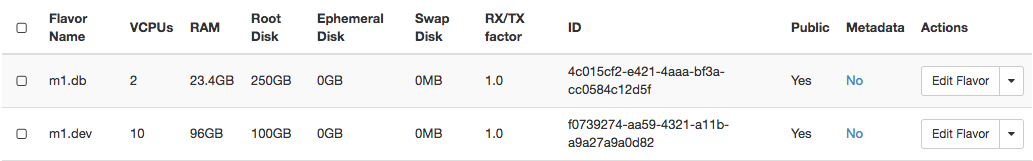
\includegraphics[scale=0.40]{img/flavors}
  \caption{List of custom created flavors to run the analytic engine
instances.}
  \label{fig:flavors}
\end{figure}

After the environment setup and configuration we uploaded a RHEL 7.3
QCOW2 image as our base Operating System to work with. We then created
two instances, one using the m1.dev flavor and the other using the m1.db
flavor, with the RHEL 7.3 image. Each instance was placed on the internal
network, assigned the firewall rules described above, and injected with
our private key. Once each instance was running, floating IP addresses
were allocated and assigned to each of the instances allowing for
external SSH connections. An SSH configuration file was created on the
host machine and proxy machine to allow simplistic access. Using the
following configuration file, users can log into the dev machine using
\textit{ssh dev} and similarly can log into the DB machine using
\textit{ssh db}.

\begin{lstlisting}[escapechar=&]
Host dev
Hostname 10.26.10.26
User team1
PubKeyAuthentication yes
IdentityFile ~/.ssh/id_rsa

Host db
Hostname 10.26.10.25
User team1
PubKeyAuthentication yes
IdentityFile ~/.ssh/id_rsa
\end{lstlisting}

Finally the user accounts seen in the configuration file above were
configured on each of the instances and the VM's red hat subscriptions
were enabled to allow the installation of packages. The implementation
of both the database and development machines followed the steps in the
Alchemy Cookbook guide written by Meaghan Johnson~\cite{alchemy} and
the details are not repeated in this report. 
